\newpage
\section{\textbf{Diagrama Unifilar de Proteção}}

Na Figura~\ref{fig:diagrama_unifilar_protecao} foi apresentada a configuração proposta para a proteção da SE Campus do Pici. Foram representados os equipamentos de manobra, os transformadores de corrente (TCs) e as funções de proteção identificadas por sua nomenclatura ANSI/IEEE C37.2. As cores distinguiram o setor de 69~kV (vermelho), o setor de 13,8~kV (azul) e a proteção dos transformadores de potência (magenta). O diagrama reuniu funções disponíveis nos vãos; sua representação não significou que todas tivessem sido habilitadas no mesmo grupo de ajustes.

\begin{figure}[htbp]
    \centering
    \caption{Diagrama unifilar de proteção da SE Campus do Pici.}
    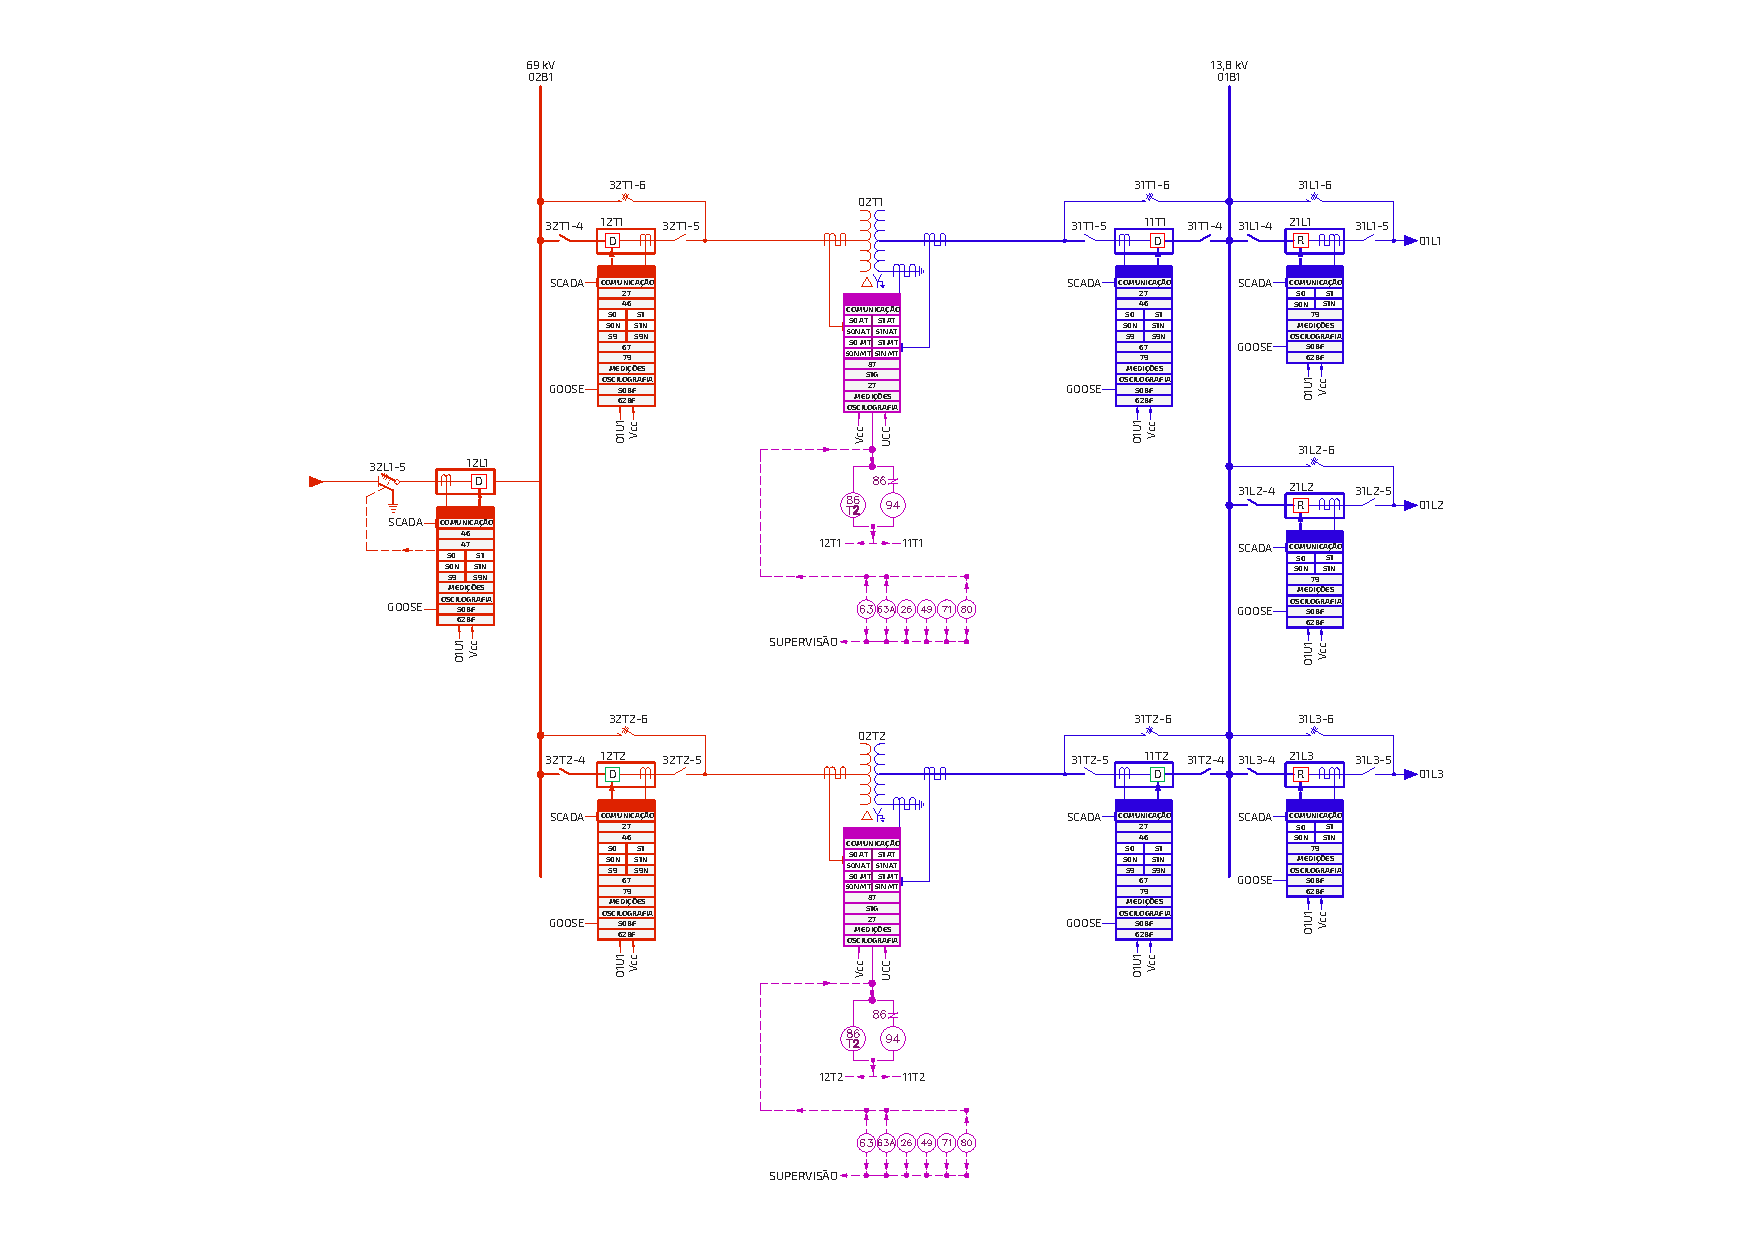
\includegraphics[width=16cm]{Imagens/Diagrama SEP.pdf}
    \label{fig:diagrama_unifilar_protecao}
    {\small Fonte: Elaborado pelos autores.}
\end{figure}

No setor de 69~kV, a entrada de linha foi associada ao disjuntor 12L1 e à chave seccionadora 32L1-5, com lâmina de aterramento. Foram representadas as funções de sobrecorrente de fase e de neutro (50/51 e 50N/51N), desequilíbrio de corrente (46), sequência de fase de tensão (47), sobretensão (59/59N) e falha de disjuntor (50BF/62BF). O barramento 02B1 foi associado aos transformadores 02T1 e 02T2 por meio dos disjuntores 12T1 e 12T2, incorporados à proposta, e de suas seccionadoras de isolamento e de \textit{by-pass}. Foram mantidas apenas as funções habilitadas nas OAPs calculadas. Em particular, os estágios 50/50N da entrada foram desabilitados no grupo estudado, e o religamento automático dos vãos dos transformadores não foi habilitado.

Para cada transformador foi prevista proteção diferencial (87T) com medição nos dois lados, conforme a especificação da seção correspondente. A proteção de sobrecorrente de retaguarda foi associada aos IEDs dos respectivos vãos, e a função 51G foi associada ao TC dedicado do neutro do enrolamento em estrela aterrada. Foi prevista a abertura dos disjuntores dos dois lados da unidade protegida, 12T1/11T1 ou 12T2/11T2, para atuação diferencial ou das proteções intrínsecas com comando de desligamento. O bloqueio 86T foi utilizado para impedir reenergização após atuação das proteções selecionadas. A função 94 foi identificada como função auxiliar de disparo, distinta do circuito de antibombeamento. Os dispositivos intrínsecos representados no diagrama não foram objeto de cálculo de ajustes elétricos neste estudo.

No setor de 13,8~kV, os transformadores foram associados ao barramento 01B1 pelos disjuntores gerais 11T1 e 11T2. Foram utilizadas as funções temporizadas de fase e de neutro nos gerais, e foram desabilitados seus estágios 50/50N no grupo estudado. Desse barramento foram representadas as saídas 01L1, 01L2 e 01L3, protegidas pelos equipamentos 21L1, 21L2 e 21L3. Nos alimentadores foram considerados sobrecorrente de fase e de neutro, neutro sensível, desequilíbrio, religamento e falha de disjuntor, conforme os ajustes da seção seguinte. As chaves de \textit{by-pass} foram mantidas no diagrama, mas sua utilização não foi incluída na topologia normal de cálculo.

Foi prevista alimentação dos IEDs em corrente contínua pelo sistema de serviços auxiliares O1U1 e integração ao SCADA. Para a troca de sinais de proteção foram consideradas mensagens GOOSE entre equipamentos com interface IEC 61850 compatível, ou contatos e interfaces apropriadas nos demais casos, sem pressupor suporte nativo ao mesmo protocolo em todos os modelos. A definição dos circuitos de disparo, dos caminhos de comunicação e de seus atrasos foi vinculada ao comissionamento. Foram preservados os recursos de medição e oscilografia para análise das perturbações. O único transformador em serviço e os pontos RP1/RP2 normalmente abertos definiram a topologia radial utilizada nos cálculos.
